\documentclass[11pt,a4paper]{article}
\usepackage[utf8]{inputenc}
\usepackage[T5]{fontenc}
\usepackage[vietnamese]{babel}
\usepackage[margin=1in]{geometry}
\usepackage{amsmath,amssymb}
\usepackage{array,booktabs,tabularx}
\usepackage{enumitem}
\usepackage{graphicx}
\usepackage{xcolor}
\usepackage{hyperref}
\usepackage{tikz}
\usetikzlibrary{arrows.meta,positioning,shapes.geometric}
\usepackage{titlesec}
\usepackage{fancyhdr}
\usepackage{ragged2e}
\usepackage{float}
\usepackage[section]{placeins}
\usepackage{caption}
\usepackage{pmboxdraw}

\setlength{\parindent}{0pt}
\setlength{\parskip}{0.28\baselineskip}
\setlength{\headheight}{14pt}
\renewcommand{\arraystretch}{1.08}
\setlist[itemize]{leftmargin=1.3em, itemsep=0.1em, topsep=0.12em}
\setlist[enumerate]{leftmargin=1.7em, itemsep=0.12em, topsep=0.12em}
\hypersetup{colorlinks=true, linkcolor=blue!50!black, urlcolor=blue!50!black}
\newcolumntype{Y}{>{\RaggedRight\arraybackslash}X}

\titleformat{\section}{\large\bfseries}{\thesection.}{0.5em}{}
\titleformat{\subsection}{\normalsize\bfseries}{\thesubsection}{0.5em}{}

\pagestyle{fancy}
\fancyhf{}
\lhead{Kính thông minh hỗ trợ người khiếm thị tích hợp AI biên và thị giác máy tính}
\rhead{Báo cáo dự án}
\cfoot{\thepage}

\begin{document}

\begin{titlepage}
    \centering
    {\Large \textbf{IoT Challenge 2026 -- Smart Healthcare with Edge AI}\par}
    \vspace{1.0cm}
    {\Huge \textbf{KÍNH THÔNG MINH HỖ TRỢ NGƯỜI KHIẾM THỊ}\par}
    \vspace{0.15cm}
    {\Large \textbf{TÍCH HỢP AI BIÊN VÀ THỊ GIÁC MÁY TÍNH}\par}
    \vspace{0.8cm}
    \vspace{0.9cm}
    
\includegraphics[width=0.34\textwidth]{prism-uploads/Logo-DH-Cong-Nghe-UET.png}\par
    \vspace{1.0cm}
    \begin{tabular}{>{\bfseries}p{4cm}p{9cm}}
        Tên nhóm & Vua \\
        Thành viên & Hà Đức Khôi, Nguyễn Hương Giang, Nguyễn Minh Cát, Kiểu Nhật Linh \\
        Trường/Lớp & Trường Đại học Công nghệ - ĐHQGHN \\
        Mentor &  \\
        Ngày nộp & \today \\
    \end{tabular}
    \vfill
    {\large Báo cáo dự án công nghệ\par}
\end{titlepage}

\tableofcontents
\newpage

\section{Bối cảnh và vấn đề}
Với người khiếm thị, khó khăn trong sinh hoạt hằng ngày không chỉ là chuyện đi đường hay tránh vật cản. Trong nhiều tình huống, điều quan trọng hơn là hiểu nhanh bối cảnh môi trường xung quanh: phía trước có gì, bên trái hay bên phải có vật gì đáng chú ý, lối đi nào đang thông thoáng, trước mặt có cửa, bàn, ghế hay người đang đứng hay không. Khi thiếu những thông tin như vậy, người dùng thường phải dừng lại để thăm dò, di chuyển chậm hơn và khó đưa ra quyết định kịp thời trong không gian đang thay đổi.

Các công cụ hỗ trợ hiện nay mới giải quyết được một phần nhu cầu đó. Gậy dò đường rất hữu ích trong việc phát hiện vật cản thấp, nhưng khó phản ánh đầy đủ các chi tiết ở tầm đầu, trên mặt bàn, trên kệ, gần cửa ra vào hoặc ở hai bên người dùng. Hệ thống định vị toàn cầu (Global Positioning System -- GPS) lại phù hợp với định vị ở quy mô lớn, nhưng không đủ chi tiết để trả lời những câu hỏi rất thực tế như nên đi hướng nào, bên trái có chướng ngại không, hay món đồ cần tìm đang nằm ở phía nào. Vì vậy, nhu cầu đặt ra là một hệ thống có thể quan sát môi trường gần, hiểu ngữ cảnh không gian và phản hồi lại bằng âm thanh theo cách ngắn gọn, dễ hiểu và dùng được ngay.

Từ nhu cầu đó, dự án định hướng xây dựng một hệ thống hỗ trợ người khiếm thị bằng cách kết hợp giọng nói và thị giác máy tính trong cùng một phiên tương tác. Hệ thống không chỉ hướng tới hỗ trợ di chuyển, nhận biết vật cản và mô tả bối cảnh xung quanh, mà còn phục vụ hỏi đáp với vision, hỗ trợ tìm và lấy đồ thuận tiện hơn trong sinh hoạt hằng ngày. Chẳng hạn, người dùng có thể hỏi trước mặt có gì, bên nào đang trống, chai nước nằm ở đâu, hay nên với tay theo hướng nào để lấy được đồ vật cần thiết. Cách tiếp cận này giúp việc tương tác với môi trường trở nên chủ động hơn, giảm phụ thuộc vào người hỗ trợ trong những việc nhỏ hằng ngày, đồng thời tạo ra một bài toán kỹ thuật phù hợp với phạm vi của một nguyên mẫu nghiên cứu và trình diễn.

\section{Mục tiêu dự án}
Mục tiêu tổng quát của dự án là xây dựng một nguyên mẫu kính thông minh có thể hỗ trợ người khiếm thị trong các nhu cầu gần và thường gặp hằng ngày, thay vì chỉ tập trung vào một chức năng đơn lẻ. Cụ thể, hệ thống hướng tới bốn nhóm hỗ trợ chính: hiểu bối cảnh môi trường xung quanh, hỏi đáp về cảnh vật bằng vision, tìm và hỗ trợ lấy đồ, và gợi ý hướng di chuyển an toàn trong phạm vi gần. Để hiện thực hóa mục tiêu đó, nguyên mẫu được triển khai trên bốn thành phần đã chốt: EFR32xG26 cho giọng nói biên, ESP32-CAM cho thị giác, gateway Android cho điều phối phiên và AI server cho xử lý nặng.

Mục tiêu kỹ thuật của dự án là hoàn thiện một chuỗi xử lý khép kín, trong đó người dùng có thể ra lệnh bằng giọng nói, hệ thống chụp ảnh đúng thời điểm, đồng bộ dữ liệu theo từng phiên và tạo phản hồi âm thanh theo cách ngắn gọn, dễ hiểu. Trọng tâm triển khai nằm ở bốn khối chính: phát hiện từ khóa đánh thức và xác định điểm kết thúc câu lệnh trên EFR32xG26; cung cấp ảnh qua máy chủ thị giác HTTP trên ESP32-CAM; quản lý \texttt{session\_id} và \texttt{timestamp} trên gateway Android; xử lý nhận dạng giọng nói, phát hiện vật thể và phân tích hình ảnh trên AI server. Trong đó, mô hình ngôn ngữ -- thị giác (VLM) giữ vai trò quan trọng trong việc kết hợp nội dung câu hỏi của người dùng với ảnh thu được để suy ra ngữ cảnh phù hợp, trả lời các câu hỏi về cảnh vật, mô tả vị trí trái -- phải, hỗ trợ tìm đồ và gợi ý hướng đi ngắn hạn. Sau khi có kết quả, phản hồi được gửi ngược lại qua BLE để EFR32xG26 phát âm thanh cho người dùng. Mục tiêu cuối cùng của nguyên mẫu là tạo ra một trải nghiệm tương tác liền mạch từ lúc người dùng gọi ``Hey Tèo'' đến khi nhận được phản hồi âm thanh phù hợp với ngữ cảnh thực tế.

Để thể hiện rõ ý đồ triển khai, các mục tiêu dưới đây được nhóm theo từng khối kỹ thuật chính của hệ thống thay vì chỉ liệt kê theo chức năng tổng quát.

\begin{table}[H]
\centering
\caption{Mục tiêu kỹ thuật theo từng khối triển khai.}
\begin{tabularx}{\textwidth}{p{3.1cm}Y Y}
\toprule
\textbf{Khối kỹ thuật} & \textbf{Trọng tâm triển khai} & \textbf{Kết quả mong đợi} \\
\midrule
Kiến trúc hệ thống & Hoàn thiện kiến trúc nhiều nút gồm EFR32xG26, ESP32-CAM, gateway Android và AI server trong cùng một luồng xử lý thống nhất & Nguyên mẫu hoạt động đồng bộ từ lúc nhận lệnh đến lúc phát phản hồi  \\
AI biên giọng nói & Phát hiện từ khóa đánh thức, ghi nhận câu lệnh và xác định điểm kết thúc câu nói trên EFR32xG26 & Node giọng nói hoạt động ổn định, mở phiên đúng lúc và gửi dữ liệu gọn, đúng ngữ cảnh  \\
Truyền thông và đồng bộ & Duy trì kết nối BLE hai chiều giữa EFR32xG26 và gateway Android, gọi HTTP từ gateway Android tới ESP32-CAM để lấy ảnh, đồng thời chỉ gateway Android gửi request hợp nhất lên AI server và quản lý \texttt{session\_id}, \texttt{timestamp} cho từng phiên & Dữ liệu giọng nói, hình ảnh, yêu cầu gửi lên AI server và phản hồi âm thanh được ghép đúng phiên, giảm lệch ngữ cảnh khi xử lý  \\
Thị giác và VLM & Cung cấp ảnh qua máy chủ thị giác HTTP trên ESP32-CAM và kết hợp ảnh với nội dung câu hỏi của người dùng để VLM suy luận, mô tả cảnh, hỏi đáp, tìm/lấy đồ và hỗ trợ định hướng gần & Hệ thống hiểu được bối cảnh xung quanh theo đúng truy vấn và sinh phản hồi phù hợp với từng nhu cầu thực tế  \\
Trình diễn nguyên mẫu & Thể hiện rõ trạng thái BLE, HTTP, AI server và luồng phản hồi âm thanh trả về EFR32xG26 trong các kịch bản hỏi đáp vision, tìm/lấy đồ và điều hướng gần & Chuỗi demo rõ ràng, dễ theo dõi, có thể lặp lại và đánh giá được  \\
\bottomrule
\end{tabularx}
\end{table}

\section{Giải pháp đề xuất và luồng sử dụng}
Giải pháp của hệ thống được tổ chức theo kiến trúc bốn thành phần, trong đó mỗi khối đảm nhiệm một vai trò riêng nhưng liên kết chặt chẽ trong cùng một phiên tương tác. EFR32xG26 phụ trách nhận biết từ khóa đánh thức, thu câu lệnh thoại và phát phản hồi âm thanh cho người dùng. ESP32-CAM cung cấp ảnh hiện trường qua HTTP nội bộ cho gateway Android. Gateway Android là một ứng dụng Android do nhóm phát triển, giữ vai trò điều phối chính: app nhận audio từ EFR32xG26, lấy ảnh từ ESP32-CAM, gắn metadata phiên rồi gửi request hợp nhất lên AI server. Trên AI server, agent điều phối sử dụng VLM host local qua Ollama để chọn hoặc chuyển đổi giữa các state machine chuyên biệt như mô tả ngoại cảnh, hỗ trợ lấy vật thể và hướng dẫn đường đi; các mô hình ASR, YOLOE, MediaPipe và VLM cung cấp dữ liệu đầu vào để sinh phản hồi phù hợp với ngữ cảnh.

Luồng của một phiên được triển khai theo thứ tự rõ ràng. Khi EFR32xG26 phát hiện đúng từ khóa đánh thức, thiết bị phát một tiếng bíp ngắn để báo bắt đầu ghi âm. Câu lệnh thoại được thu cho đến khi mức âm thanh giảm xuống dưới ngưỡng kết thúc trong một khoảng thời gian đủ dài; lúc đó thiết bị phát thêm một tiếng bíp nữa để báo dừng ghi âm và gửi dữ liệu thoại qua BLE cho app gateway Android. App Android sau đó gọi \texttt{/capture} để lấy ảnh từ ESP32-CAM, gắn \texttt{session\_id} cùng các mốc thời gian, rồi gửi request hợp nhất qua HTTP lên AI server. EFR32xG26 và ESP32-CAM không giao tiếp trực tiếp với AI server. Tại AI server, agent dựa trên VLM local Ollama xác định yêu cầu của người dùng và chuyển request vào state machine phù hợp. Sau khi có kết quả, phản hồi âm thanh được chuyển ngược lại qua BLE để EFR32xG26 phát ra cho người dùng.

\begin{figure}[H]
\centering
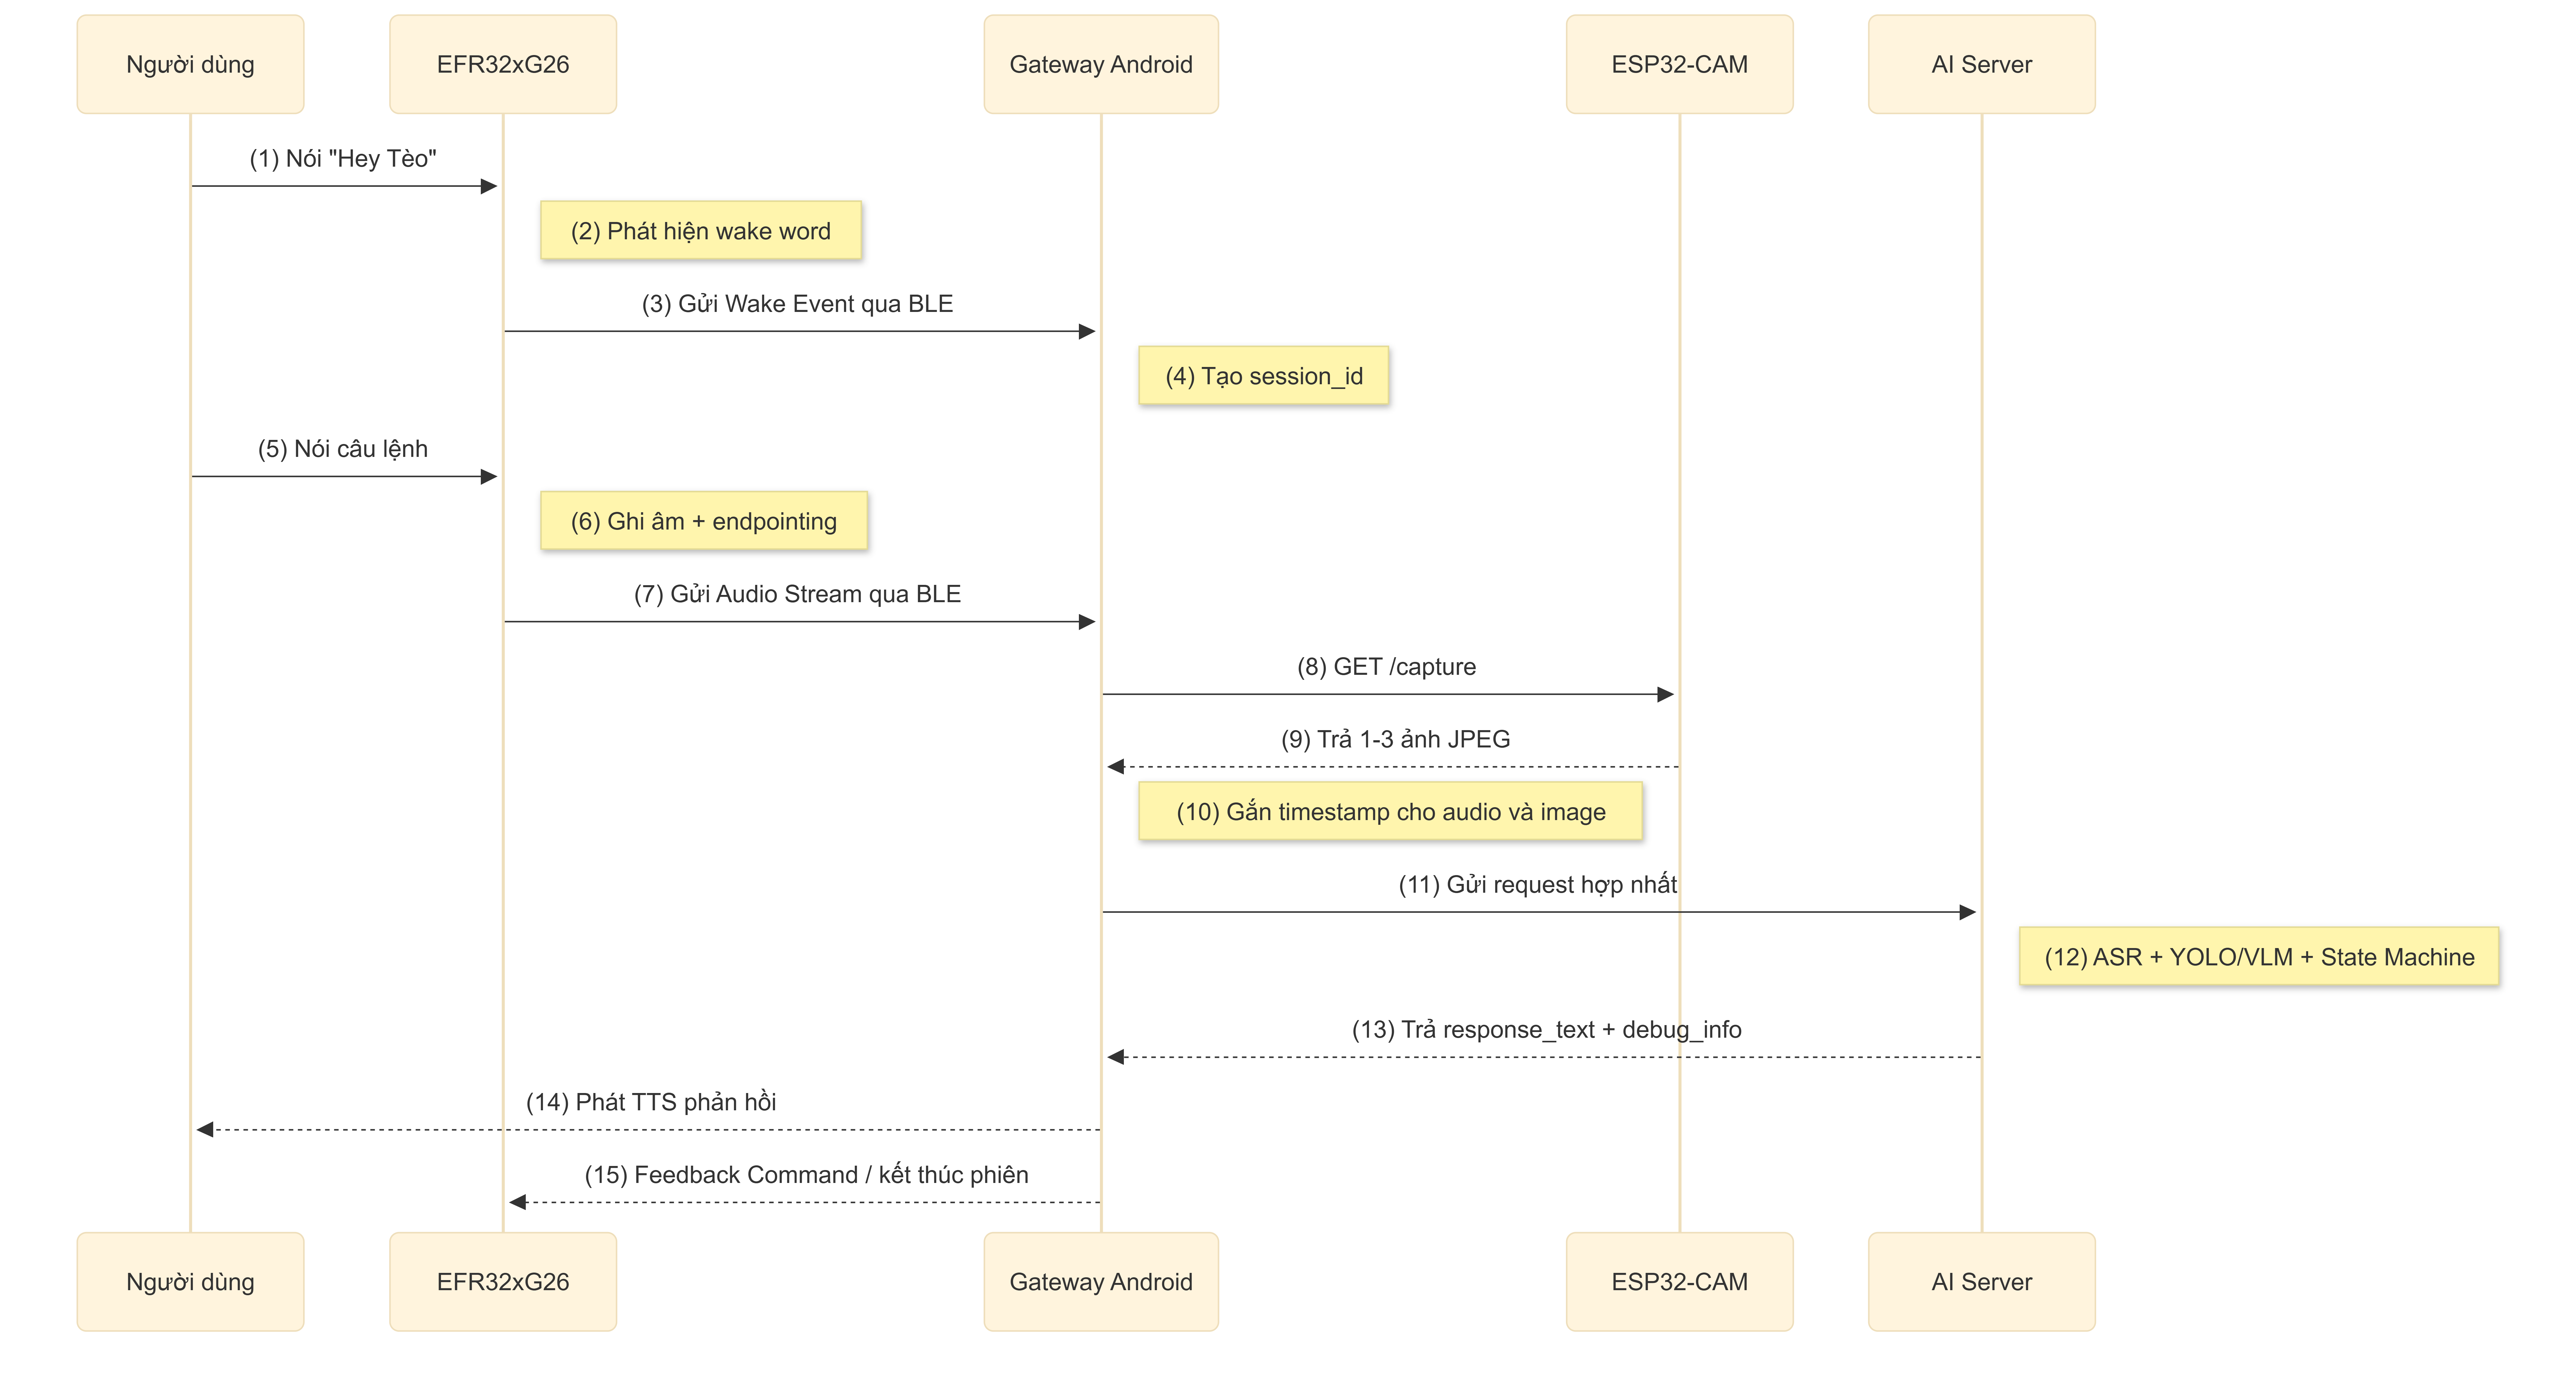
\includegraphics[width=0.96\textwidth]{prism-uploads/ESP32-CAM Audio-IMU Workflow-2026-05-11-040727_2.png}
\caption{Minh họa luồng xử lý trong phần giải pháp đề xuất và luồng sử dụng. Hình này cho thấy EFR32xG26 và ESP32-CAM đều gửi dữ liệu về gateway Android; sau đó chỉ gateway Android gửi request hợp nhất lên AI server và chuyển phản hồi âm thanh về EFR32xG26 cho người dùng.}
\end{figure}

Kịch bản thứ nhất là hỏi đáp với vision về cảnh vật phía trước. Người dùng nói ``Hey Tèo, phía trước có gì?'' hoặc ``Hey Tèo, trước mặt có cửa không?''. Node AI biên phát hiện từ khóa, mở phiên ghi âm, đóng gói câu lệnh thoại và chuyển đến gateway Android. Ứng dụng Android gọi \texttt{/capture} để lấy ảnh JPEG đúng thời điểm từ ESP32-CAM, sau đó gateway gửi audio command và ảnh lên AI server. ASR chuyển âm thanh thành văn bản; VLM kết hợp nội dung câu hỏi với ảnh để suy ra câu trả lời phù hợp; bộ điều phối tạo phản hồi cuối cùng; gateway Android chuyển phản hồi âm thanh ngược lại qua BLE để EFR32xG26 phát cho người dùng.

Kịch bản thứ hai là tìm và hỗ trợ lấy đồ vật. Người dùng nói ``Hey Tèo, tìm chai nước'' hoặc ``Hey Tèo, giúp mình lấy hộp thuốc''. Câu lệnh thoại từ EFR32xG26 và ảnh JPEG từ ESP32-CAM được gateway Android ghép cùng một phiên rồi gửi lên AI server. Trong kịch bản này, YOLOE được dùng để nhận diện đúng vật thể mục tiêu theo yêu cầu, còn MediaPipe được dùng để nhận diện bàn tay người dùng và ước lượng hướng đưa tay trong khung hình. Từ hai nguồn thông tin đó, hệ thống có thể hướng dẫn cụ thể hơn như đưa tay sang trái, sang phải, lên cao hơn, thấp xuống hoặc tiến gần thêm để chạm tới vật thể cần lấy. Khi cần, VLM bổ sung mô tả ngữ cảnh để làm rõ vật đang ở đâu so với tay người dùng. Phản hồi sau đó được chuyển qua BLE để EFR32xG26 phát lại cho người dùng.

Kịch bản thứ ba là hỗ trợ hướng dẫn đi đường trong phạm vi gần. Người dùng có thể hỏi ``Hey Tèo, đi hướng nào an toàn?'' hoặc ``Hey Tèo, có thể đi thẳng không?''. Trong trường hợp này, VLM không chỉ mô tả ảnh đơn lẻ mà còn kết hợp ảnh với câu hỏi định hướng của người dùng để khai thác ngữ cảnh không gian như khoảng trống phía trước, hướng mở của lối đi, vị trí vật cản nổi bật hoặc mép hành lang. Hệ thống từ đó sinh phản hồi ngắn gọn như ``có thể đi thẳng'', ``lệch trái một chút'' hoặc ``có vật cản phía trước, nên tránh sang phải'', rồi chuyển phản hồi đó qua BLE để EFR32xG26 phát ra cho người dùng.

\begin{table}[H]
\centering
\caption{Luồng xử lý của một phiên tương tác.}
\begin{tabularx}{\textwidth}{p{1.2cm}p{2.4cm}p{3.8cm}p{3.2cm}Y}
\toprule
\textbf{Bước} & \textbf{Tác nhân} & \textbf{Hành động} & \textbf{Dữ liệu sinh ra} & \textbf{Kết quả} \\
\midrule
1 & Người dùng & Gọi wake word và nói câu lệnh & Tín hiệu giọng nói đầu vào & Phiên tương tác được khởi tạo \\
2 & EFR32xG26 & Phát hiện wake word, mở phiên audio, endpointing & Wake event, audio command, device status & Dữ liệu giọng nói được chốt theo session \\
3 & Gateway Android & Nhận audio command qua BLE và tạo \texttt{session\_id} & Metadata phiên, timestamp & Session được quản lý tập trung \\
4 & Gateway Android & Gọi \texttt{/capture} đến ESP32-CAM & 1--3 ảnh JPEG, image timestamp & Dữ liệu thị giác được gắn vào session \\
5 & AI server & Xử lý request hợp nhất & \texttt{recognized\_text}, \texttt{detected\_objects}, \texttt{response\_text} & Kết quả xử lý đa phương thức được tạo ra \\
6 & Gateway Android + EFR32xG26 & Gateway chuyển phản hồi qua BLE, EFR32xG26 phát âm thanh & Gói phản hồi, trạng thái phiên & Session kết thúc sau khi phản hồi hoàn tất \\
\bottomrule
\end{tabularx}
\end{table}


\section{Kiến trúc hệ thống}
Ở mức kiến trúc, nguyên mẫu được chia thành bốn nút xử lý chính: nút giọng nói biên trên EFR32xG26, nút thị giác trên ESP32-CAM, gateway Android trên điện thoại và AI server cho các tác vụ tính toán nặng. Cách phân tách này giúp mỗi phần cứng đảm nhiệm một vai trò rõ ràng, đồng thời vẫn tham gia vào cùng một phiên tương tác được quản lý bằng \texttt{session\_id}.

Trong phạm vi báo cáo, thuật ngữ gateway Android được dùng thống nhất để chỉ ứng dụng trung gian chạy trên điện thoại Android. EFR32xG26 đảm nhiệm kích hoạt bằng từ khóa đánh thức, ghi nhận câu lệnh thoại, truyền dữ liệu âm thanh qua BLE về gateway và phát phản hồi âm thanh cuối cùng cho người dùng. ESP32-CAM đóng vai trò nút thị giác, cung cấp ảnh JPEG theo yêu cầu thông qua máy chủ HTTP nội bộ cho gateway. Gateway Android điều phối phiên, gắn \texttt{session\_id} và \texttt{timestamp}, hợp nhất dữ liệu âm thanh -- hình ảnh, gửi yêu cầu xử lý lên AI server qua HTTP và chuyển phản hồi trở lại EFR32xG26. Như vậy, EFR32xG26 và ESP32-CAM không gửi dữ liệu trực tiếp lên AI server; chỉ gateway Android giao tiếp với AI server. AI server thực hiện nhận dạng giọng nói, phát hiện vật thể bằng YOLOE, nhận diện bàn tay bằng MediaPipe, phân tích ngữ cảnh bằng mô hình ngôn ngữ -- thị giác và sinh nội dung phản hồi phù hợp với truy vấn của người dùng.

\begin{table}[H]
\centering
\caption{Phân tách chức năng giữa các nút trong kiến trúc hệ thống.}
\footnotesize
\setlength{\tabcolsep}{3pt}
\begin{tabularx}{\textwidth}{%
>{\hsize=0.80\hsize\RaggedRight\arraybackslash}X%
>{\hsize=0.80\hsize\RaggedRight\arraybackslash}X%
>{\hsize=1.25\hsize\RaggedRight\arraybackslash}X%
>{\hsize=0.95\hsize\RaggedRight\arraybackslash}X%
>{\hsize=1.20\hsize\RaggedRight\arraybackslash}X%
>{\hsize=1.00\hsize\RaggedRight\arraybackslash}X}
\toprule
\textbf{Lớp / Nút} & \textbf{Phần cứng} & \textbf{Chức năng chính} & \textbf{Dữ liệu vào} & \textbf{Dữ liệu ra} & \textbf{Giao thức} \\
\midrule
Nút AI biên giọng nói & EFR32xG26 Dev Kit & Phát hiện wake word, thu câu lệnh, endpointing, phát phản hồi âm thanh & Audio nền từ microphone, gói phản hồi từ gateway & Wake event, audio command, device status, audio feedback & BLE \\
Nút thị giác HTTP nội bộ & ESP32-CAM + camera & Cung cấp ảnh JPEG và trạng thái camera theo yêu cầu & HTTP request từ gateway Android & JPEG frame, camera status, stream debug & HTTP trên Wi-Fi nội bộ \\
Gateway Android & Điện thoại Android & Quản lý session, đồng bộ audio-image, gọi AI server, chuyển phản hồi về EFR32xG26 & Wake event, audio command, JPEG frame & Request hợp nhất, gói phản hồi, feedback status & BLE, HTTP, Wi-Fi/Internet \\
Nút AI server & Máy tính / laptop chạy AI server & Xử lý ASR, YOLO/VLM và điều phối phản hồi & Audio + image + metadata phiên từ gateway Android & \texttt{recognized\_text}, \texttt{detected\_objects}, \texttt{response\_text} & API với gateway Android trên Wi-Fi/Internet \\
\bottomrule
\end{tabularx}
\end{table}

\begin{figure}[H]
\centering
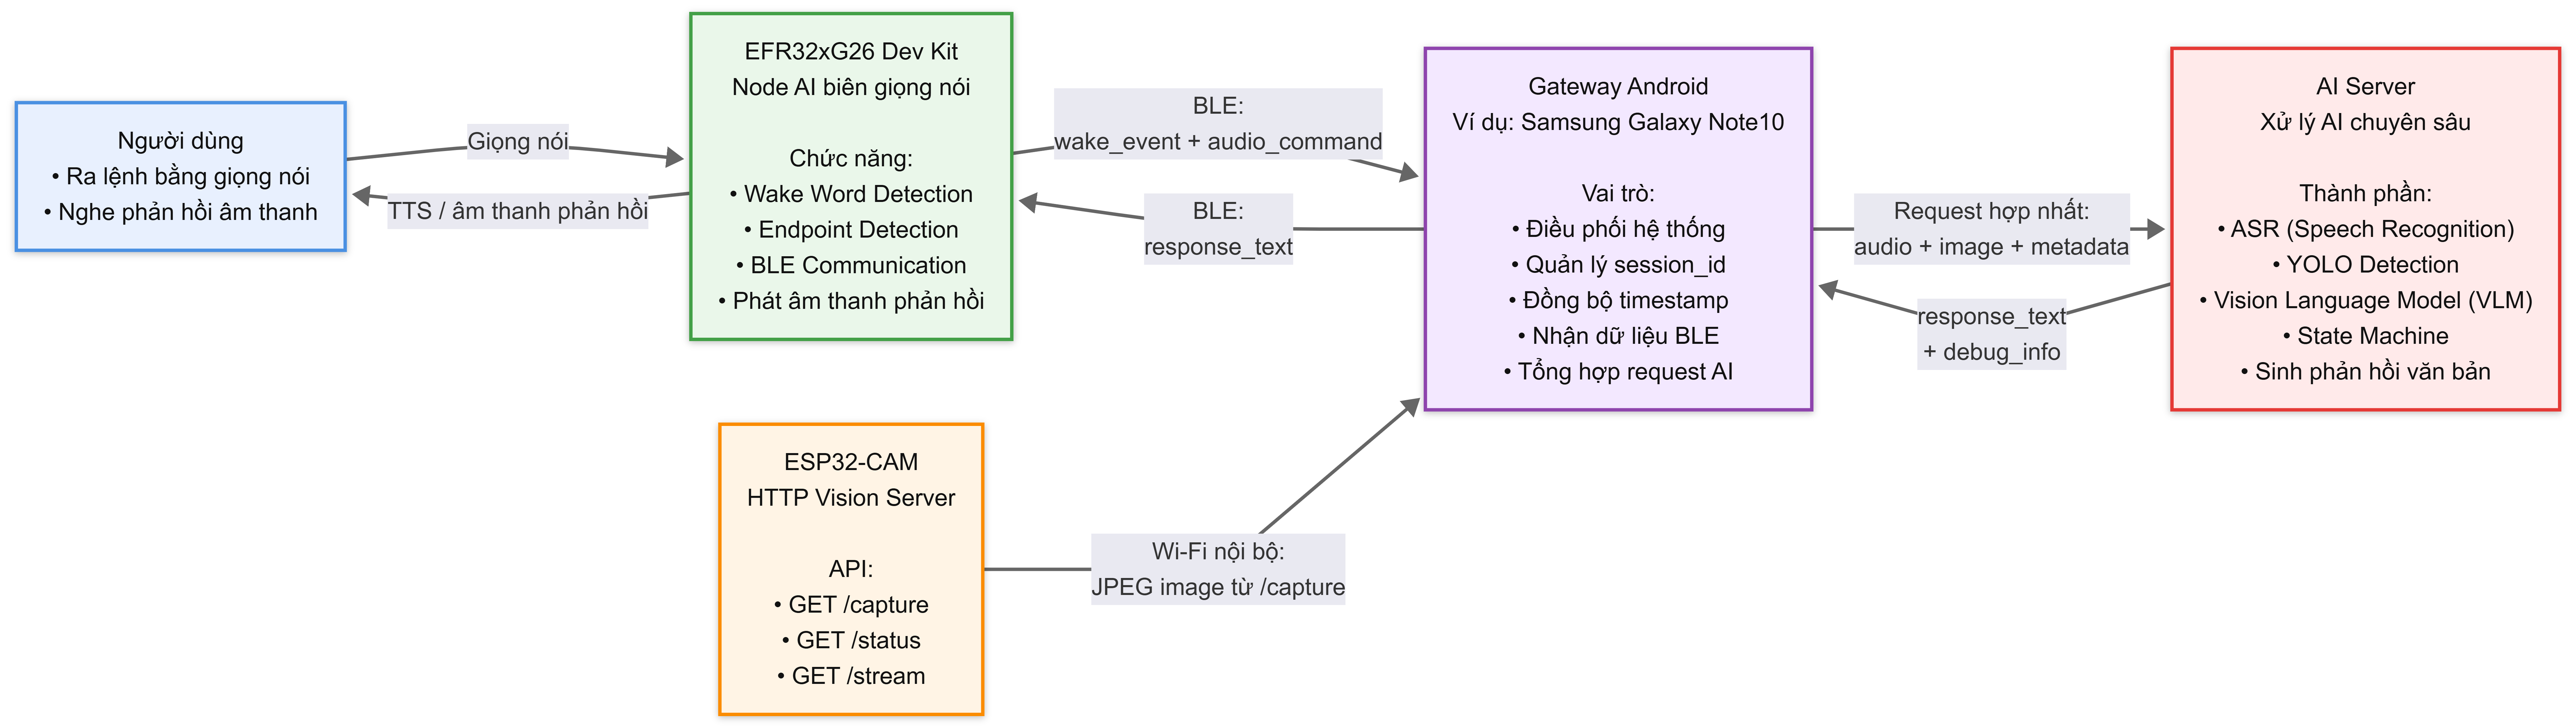
\includegraphics[width=0.88\textwidth]{uploads/so_do_2.png}
\caption{Sơ đồ kiến trúc tổng thể của hệ thống. EFR32xG26 gửi dữ liệu giọng nói qua BLE về gateway Android, ESP32-CAM cung cấp ảnh qua HTTP Vision Server cho gateway Android, còn gateway Android là thành phần duy nhất gửi request hợp nhất lên AI server để xử lý ASR, YOLO/VLM và điều phối phản hồi.}
\end{figure}

\subsection{Xử lý giọng nói bằng AI biên trên EFR32xG26}
EFR32xG26 Dev Kit là nút AI biên phụ trách toàn bộ đường giọng nói tại thiết bị đeo. Mục tiêu của nút này không phải là xử lý ngôn ngữ hoàn chỉnh, mà là nhận biết đúng thời điểm người dùng gọi hệ thống, thu câu lệnh sau wake word, xác định điểm kết thúc câu nói và truyền dữ liệu âm thanh đã đóng gói sang gateway Android. Cách tổ chức này giúp thiết bị không phải gửi audio liên tục, giảm tải truyền thông và vẫn giữ được phản hồi tương tác tự nhiên cho người dùng.

Mô hình wake word được huấn luyện riêng cho cụm kích hoạt ``Hey Tèo'' theo bài toán keyword spotting nhị phân. Dataset được tổ chức theo cách tương tự định dạng Google Speech Commands v2 và các ví dụ audio classification cho xG26 của Silicon Labs: mỗi lớp dữ liệu là một thư mục riêng, trong đó \texttt{hey\_teo} là lớp từ khóa mục tiêu, \texttt{\_unknown\_} chứa các mẫu không phải wake word và hard-negative, còn \texttt{\_silence\_} chứa silence/background noise.

\begin{center}
\begin{minipage}{0.86\textwidth}
\small
\begin{verbatim}
dataset/
├── hey_teo/
│   ├── sample001.wav
│   ├── sample002.wav
│   └── ...
├── _unknown_/
│   ├── neg001.wav
│   ├── neg002.wav
│   └── ...
└── _silence_/
    ├── noise001.wav
    ├── noise002.wav
    └── ...
\end{verbatim}
\end{minipage}
\end{center}

Trong đó, \texttt{hey\_teo} gồm các đoạn có chứa ``Hey Tèo'' hoặc biến thể gần như ``Hey Tèo ơi''; \texttt{\_unknown\_} gồm hội thoại thông thường, tiếng nói từ TV/Youtube và các từ gần âm như ``hey'', ``tèo'', ``theo'', ``hello''; còn \texttt{\_silence\_} gồm tiếng quạt, tiếng lớp học, tiếng xe, tiếng gió, white noise hoặc các đoạn im lặng. Việc bổ sung hard-negative samples trong \texttt{\_unknown\_} đặc biệt quan trọng vì tiếng Việt có dấu thanh, nhiều âm gần nhau và khác biệt vùng miền, dễ làm mô hình kích hoạt nhầm nếu chỉ huấn luyện bằng dữ liệu sạch.

Dữ liệu thu âm được chuẩn hóa đúng về mono PCM 16-bit WAV, sample rate 16 kHz và độ dài khoảng 1--2 giây cho mỗi mẫu để phù hợp pipeline keyword spotting trên EFR32xG26. Nguồn thu gồm điện thoại, microphone laptop và microphone dùng với EFR32xG26 để tăng độ tương đồng với môi trường triển khai thật. Trong quá trình chuẩn bị dữ liệu, nhóm áp dụng các bước tăng cường như thêm nhiễu nền, dịch thời gian, thay đổi nhẹ cao độ hoặc tốc độ nói, đồng thời cân bằng dữ liệu giữa \texttt{hey\_teo}, \texttt{\_unknown\_} và \texttt{\_silence\_} để mô hình không thiên lệch về một lớp.

\begin{figure}[H]
\centering
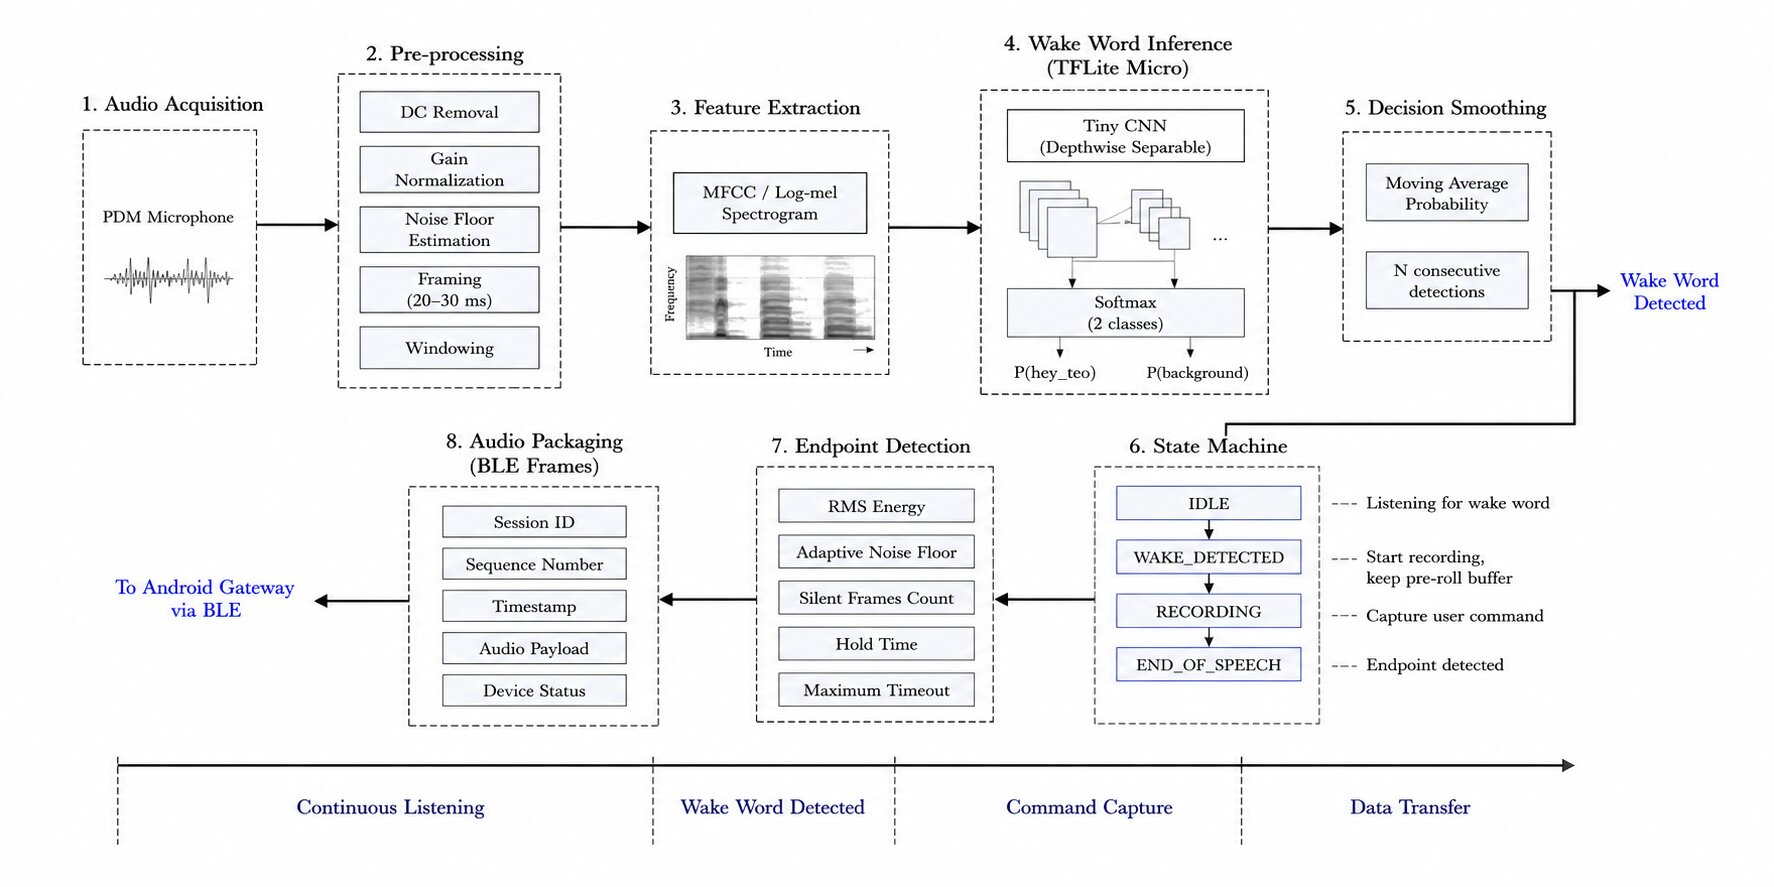
\includegraphics[width=0.94\textwidth]{uploads/so_do_3.jpg}
\caption{Pipeline huấn luyện và triển khai wake word ``Hey Tèo'' trên EFR32xG26. Hình minh họa chuỗi xử lý từ tổ chức dataset theo cấu trúc Speech Commands, trích xuất đặc trưng MFCC/log-mel, huấn luyện mô hình keyword spotting, lượng tử hóa INT8 đến suy luận thời gian thực trên firmware.}
\end{figure}

Trước khi đưa vào mô hình TinyML, tín hiệu âm thanh được chia thành các frame ngắn khoảng 20--30 ms và chuyển thành đặc trưng phổ MFCC/log-mel spectrogram theo cấu hình của pipeline huấn luyện. Các đặc trưng này là đầu vào của mô hình keyword spotting gọn, sử dụng Depthwise Separable CNN, Dense layer và Softmax hai lớp gồm \texttt{background} và \texttt{hey\_teo}. Quá trình huấn luyện được thực hiện bằng TensorFlow/Keras, TensorFlow Lite và Silicon Labs Machine Learning Toolkit; sau đó mô hình được đánh giá ở dạng TFLite để kiểm tra độ chính xác, tỷ lệ false positive và false negative trước khi đưa xuống thiết bị.

Sau khi đạt chất lượng mong muốn, mô hình được lượng tử hóa INT8 để giảm Flash, RAM và độ trễ, rồi chuyển file \texttt{.tflite} thành mảng C/C++ nhúng vào firmware EFR32xG26. Khi chạy thực tế, firmware lấy mẫu microphone, trích xuất MFCC/log-mel và suy luận bằng TFLite Micro để tính xác suất wake word; kết quả được làm ổn định bằng moving average hoặc yêu cầu nhiều lần vượt ngưỡng liên tiếp trước khi chuyển từ \texttt{IDLE} sang \texttt{WAKE\_DETECTED}. Sau tín hiệu bắt đầu ghi âm, thiết bị giữ pre-roll buffer, chuyển sang \texttt{RECORDING}, dùng endpointing dựa trên năng lượng, noise floor, số frame im lặng, hold time và timeout để xác định \texttt{END\_OF\_SPEECH}, rồi chia audio command thành các BLE frame có \texttt{sequence\_number} và gửi kèm device status sang gateway Android để đồng bộ với ảnh ESP32-CAM trước khi tạo request AI.


\subsection{Giao thức truyền thông và HTTP Vision Server}

Hệ thống sử dụng kiến trúc truyền thông đa tầng: BLE truyền audio command từ EFR32xG26 với năng lượng thấp, HTTP nội bộ lấy ảnh JPEG từ ESP32-CAM, còn gateway Android điều phối session, ghép dữ liệu đa phương thức và là thành phần duy nhất gửi request lên AI server. Cách tách tuyến này giúp các node biên hoạt động độc lập nhưng vẫn đồng bộ theo từng phiên, đồng thời tập trung quản lý timestamp, session state, retry policy và logging tại gateway.

\begin{figure}[H]
\centering
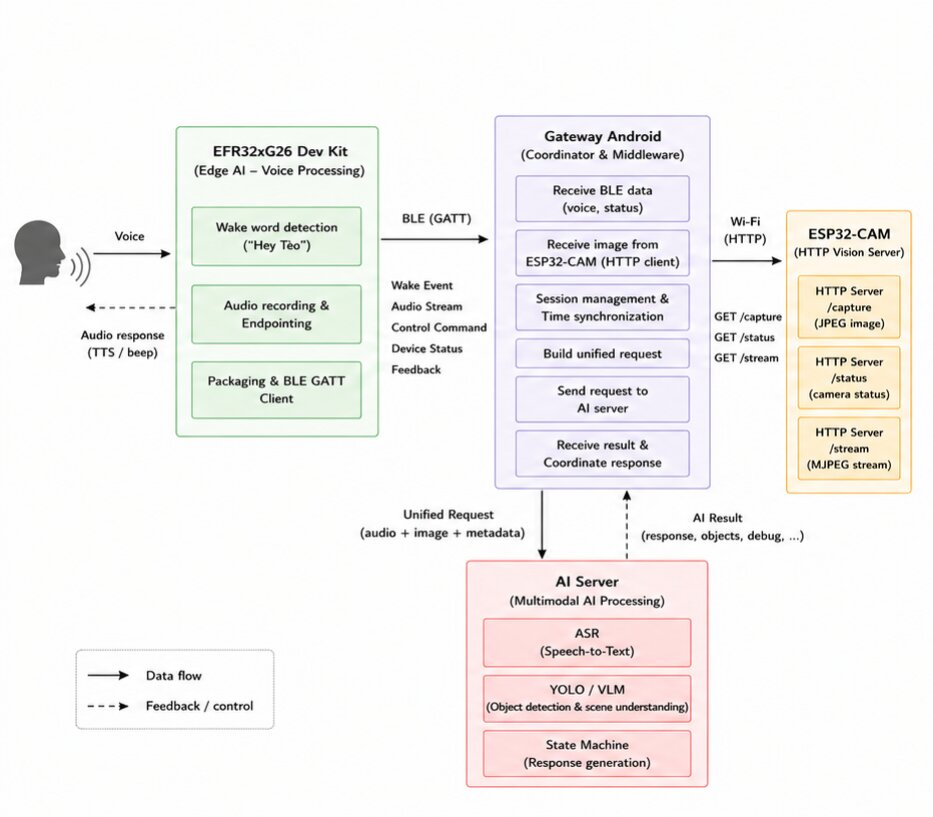
\includegraphics[width=0.80\textwidth]{uploads/so_do_5.jpg}
\caption{Kiến trúc truyền thông đa tầng của hệ thống. EFR32xG26 và ESP32-CAM chỉ trao đổi dữ liệu với gateway Android; gateway là đầu mối duy nhất tạo request hợp nhất và giao tiếp với AI server.}
\end{figure}

\subsubsection{BLE GATT giữa EFR32xG26 và gateway Android}

Kênh BLE giữa EFR32xG26 và gateway Android được xây dựng theo mô hình BLE GATT Service nhằm tối ưu cho giao tiếp công suất thấp và truyền dữ liệu ngắt quãng theo sự kiện. Thay vì streaming microphone liên tục, node AI biên chỉ truyền dữ liệu khi wake word được xác nhận và audio command đã được ghi nhận. Cách tiếp cận event-driven này giúp giảm tiêu thụ năng lượng, giảm tải BLE bandwidth và tăng tính riêng tư cho người dùng.

Các characteristic được tách riêng theo vai trò chức năng để đơn giản hóa quá trình kiểm thử, debug và quản lý vòng đời session. Trong đó, Wake Event được dùng để khởi tạo phiên tương tác; Audio Stream truyền audio command theo từng BLE frame; Control quản lý trạng thái phiên; Device Status giám sát trạng thái node AI biên; và Feedback Command cho phép gateway phản hồi kết quả xử lý về thiết bị đeo.

Đối với Audio Stream, audio command được phân mảnh thành nhiều BLE packet nhỏ nhằm phù hợp với giới hạn MTU của BLE. Mỗi packet chứa \texttt{sequence\_number}, timestamp và payload length để hỗ trợ phát hiện mất gói, sắp xếp lại thứ tự frame và ghi log debug. Gateway Android thực hiện packet reassembly trước khi tạo audio blob hoàn chỉnh cho AI server.

\begin{figure}[H]
\centering
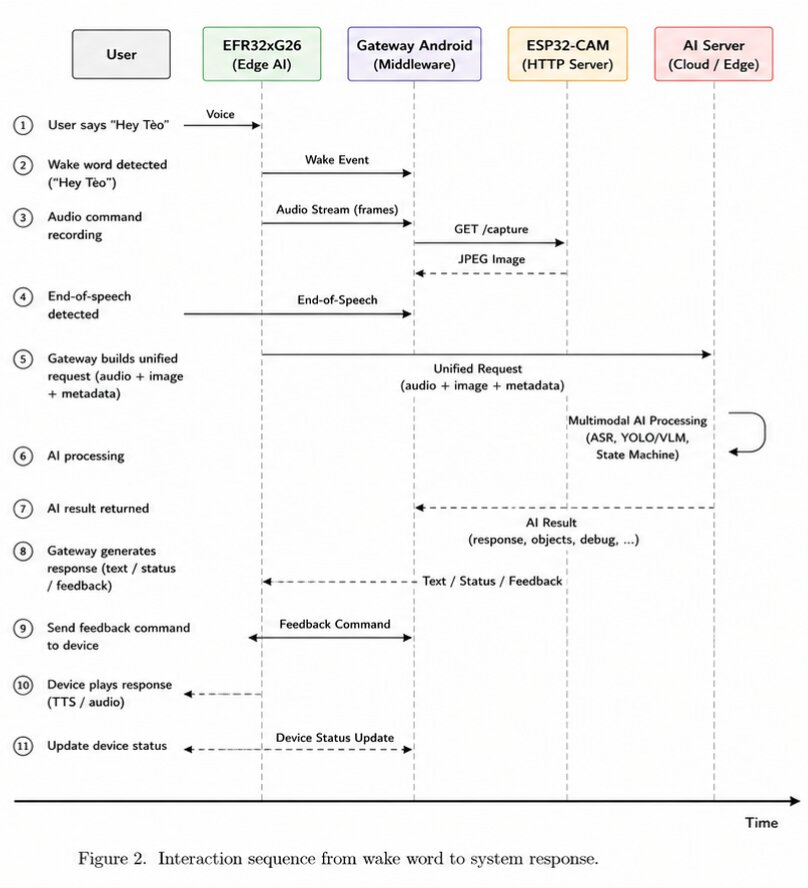
\includegraphics[width=0.76\textwidth]{uploads/so_do_4.jpg}
\caption{Vòng đời session tại gateway Android. Gateway nhận audio command từ EFR32xG26, lấy ảnh JPEG từ ESP32-CAM, gắn metadata thời gian, gửi request hợp nhất lên AI server và chuyển phản hồi về thiết bị đeo qua BLE.}
\end{figure}

\subsubsection{HTTP Vision Server trên ESP32-CAM}

ESP32-CAM hoạt động như một vision node độc lập trong mạng nội bộ và cung cấp dữ liệu ảnh theo cơ chế request-response. Thiết bị được cấu hình ở chế độ Wi-Fi station và kết nối vào hotspot của gateway Android hoặc router nội bộ để giảm độ trễ truyền ảnh.


Sau khi khởi tạo camera driver và kết nối mạng thành công, ESP32-CAM tạo HTTP Vision Server với ba endpoint chính: \texttt{/capture}, \texttt{/status} và \texttt{/stream}. Trong đó, endpoint \texttt{/capture} đóng vai trò quan trọng nhất trong pipeline AI vì cung cấp một frame JPEG tại đúng thời điểm gateway yêu cầu. Điều này giúp hệ thống đồng bộ ảnh với audio command theo từng session thay vì duy trì video streaming liên tục.

Endpoint \texttt{/status} cho phép gateway Android kiểm tra trạng thái hoạt động của vision node như camera readiness, FPS hiện tại, heap usage hoặc Wi-Fi RSSI trước khi gửi request AI. Endpoint \texttt{/stream} cung cấp MJPEG stream phục vụ quan sát trực tiếp và debug trong quá trình phát triển, tuy nhiên không thuộc luồng xử lý AI chính do tiêu tốn băng thông lớn hơn.



\subsubsection{Request hợp nhất từ gateway Android đến AI server}

Gateway Android là ứng dụng Android do nhóm phát triển và là lớp điều phối chính của toàn bộ hệ thống. Sau khi nhận đủ audio command từ EFR32xG26 và ảnh JPEG từ ESP32-CAM, app tạo request hợp nhất cho từng session trước khi gửi lên AI server.

Request được tổ chức theo hướng đa phương thức (multimodal request), bao gồm metadata phiên, audio command và image payload trong cùng một ngữ cảnh thời gian. Các trường dữ liệu quan trọng gồm \texttt{session\_id}, \texttt{wake\_timestamp}, \texttt{audio\_start\_timestamp}, \texttt{audio\_end\_timestamp}, \texttt{image\_timestamp}, audio blob, JPEG image và \texttt{device\_status}. Nhờ cấu trúc này, AI server đồng bộ chính xác giữa lời nói của người dùng và trạng thái cảnh vật tại cùng thời điểm.

Trên AI server, agent sử dụng VLM host local qua Ollama để đọc nội dung câu hỏi, ảnh và metadata phiên, sau đó chọn state machine phù hợp cho từng nhóm yêu cầu như hỗ trợ lấy vật thể, hướng dẫn đường đi hoặc mô tả ngoại cảnh. Sau khi state machine tương ứng xử lý xong, AI server trả về văn bản nhận dạng, kết quả thị giác, nội dung phản hồi, mức ưu tiên và thông tin debug; app gateway Android dùng kết quả này để gửi phản hồi về EFR32xG26 qua BLE và kết thúc session.

\subsubsection{Đồng bộ thời gian và quản lý session}

Mỗi phiên tương tác được định danh bằng \texttt{session\_id} do gateway Android tạo ngay sau khi wake event được xác nhận. Gateway đóng vai trò nguồn thời gian trung tâm của hệ thống nhằm tránh sai lệch timestamp giữa các node AI biên.

Các mốc thời gian quan trọng như wake timestamp, audio start, audio end và image capture time đều được ghi nhận tại gateway Android để tạo một hệ quy chiếu thời gian thống nhất. Điều này đặc biệt quan trọng đối với các truy vấn đa phương thức cần liên kết giữa lời nói và khung hình tương ứng.

Để tăng tính ổn định, gateway chỉ gửi request AI khi cả audio command và JPEG frame hợp lệ đã sẵn sàng. Nếu endpoint \texttt{/capture} lỗi hoặc timeout, gateway thực hiện retry theo số lần giới hạn. Trong trường hợp BLE audio thiếu frame hoặc mất packet, session được đánh dấu \texttt{incomplete} trong debug log nhằm phục vụ kiểm tra và phân tích lỗi sau quá trình demo hoặc thử nghiệm hệ thống.

\subsection{Thành phần phần cứng}

Kiến trúc phần cứng của hệ thống được thiết kế theo hướng phân tách rõ ràng giữa các chức năng giọng nói, thị giác, điều phối phiên và xử lý AI nhằm giảm tải cho thiết bị đeo và tăng khả năng mở rộng của nguyên mẫu. Trong đó, EFR32xG26 đảm nhiệm AI biên cho đường giọng nói, ESP32-CAM phụ trách dữ liệu thị giác, gateway Android điều phối session đa phương thức và AI server thực hiện các tác vụ suy luận chuyên sâu.

\begin{table}[H]
\centering
\caption{Danh sách thành phần phần cứng và vai trò trong nguyên mẫu.}
\begin{tabularx}{\textwidth}{p{0.7cm}p{3.2cm}p{4.4cm}p{3.2cm}Y}
\toprule
\textbf{STT} & \textbf{Thành phần} & \textbf{Vai trò trong hệ thống} & \textbf{Giao tiếp / dữ liệu chính} & \textbf{Trạng thái} \\
\midrule

1 &
EFR32xG26 Dev Kit &
Nút AI biên xử lý wake word, endpointing, BLE audio và phản hồi âm thanh &
Wake event, audio command, BLE GATT, I2S audio &
Có sẵn \\

2 &
Stereo MEMS microphone
(ICS-43434 trên xG26) &
Thu nhận tín hiệu giọng nói cho pipeline TinyML &
Audio PCM 16 kHz đưa trực tiếp vào firmware inference &
Tích hợp sẵn trên board \\

3 &
MAX98357A I2S Amplifier &
Giải mã và khuếch đại tín hiệu âm thanh phản hồi &
I2S audio từ EFR32xG26 tới loa &
Có sẵn \\

4 &
ESP32-CAM &
HTTP Vision Server và node thị giác của hệ thống &
JPEG image, HTTP endpoint \texttt{/capture}, \texttt{/status}, \texttt{/stream} &
Có sẵn \\

5 &
Camera OV2640
(tích hợp trên ESP32-CAM) &
Thu nhận hình ảnh môi trường phía trước người dùng &
Khung hình camera nội bộ cho ESP32-CAM &
Tích hợp sẵn trên board \\

6 &
Gateway Android
(nguyên mẫu: Samsung Galaxy Note10) &
Ứng dụng Android điều phối session và đồng bộ dữ liệu đa phương thức &
BLE với xG26, HTTP với ESP32-CAM, Wi-Fi/Internet với AI server &
Có sẵn \\

7 &
AI Server &
Chạy ASR, YOLO/VLM, agent Ollama và các state machine theo tác vụ &
Request hợp nhất, VLM local qua Ollama, GPU/CPU server &
Có sẵn \\

8 &
ICM-40627 6-axis IMU
(tích hợp trên xG26) &
Thu thập dữ liệu quán tính phục vụ hướng mở rộng contextual awareness &
Gia tốc kế và con quay hồi chuyển &
Tích hợp sẵn trên board \\

9 &
Nguồn cấp / pin &
Cấp nguồn cho các node thiết bị đeo &
Nguồn DC nội bộ &
Đang hoàn thiện \\

10 &
Gọng kính / khung cơ khí &
Tích hợp và cố định các module phần cứng trên nguyên mẫu đeo được &
Không gian lắp ráp cơ khí &
Đang hoàn thiện \\

\bottomrule
\end{tabularx}
\end{table}

\subsection{Luồng phần mềm và AI}

Luồng phần mềm của hệ thống được tổ chức theo hướng event-driven kết hợp state machine nhằm đồng bộ hoạt động giữa AI biên, gateway Android và AI server trong từng phiên tương tác. Mỗi thành phần chỉ đảm nhiệm một nhóm chức năng riêng, giúp hệ thống dễ kiểm thử, mở rộng và debug trong quá trình phát triển.

Ở trạng thái \texttt{IDLE}, EFR32xG26 liên tục chạy mô hình TinyML để phát hiện wake word ``Hey Tèo''. Khi wake word được xác nhận, state machine chuyển sang \texttt{WAKE\_DETECTED} và gửi wake event tới gateway Android thông qua BLE GATT.

Sau đó, hệ thống chuyển sang trạng thái \texttt{RECORDING}. EFR32xG26 bắt đầu ghi audio command, duy trì pre-roll buffer để tránh mất phần đầu câu lệnh và chia audio thành nhiều BLE frame nhỏ có \texttt{sequence\_number}. Gateway Android thực hiện packet reassembly để tạo audio hoàn chỉnh cho từng session.

Song song với luồng giọng nói, gateway Android gửi HTTP request tới ESP32-CAM thông qua endpoint \texttt{/capture} để lấy ảnh JPEG tương ứng với thời điểm người dùng phát lệnh. ESP32-CAM chỉ hoạt động như một HTTP Vision Server nội bộ và không giao tiếp trực tiếp với AI server.
\begin{figure}[H]
\centering
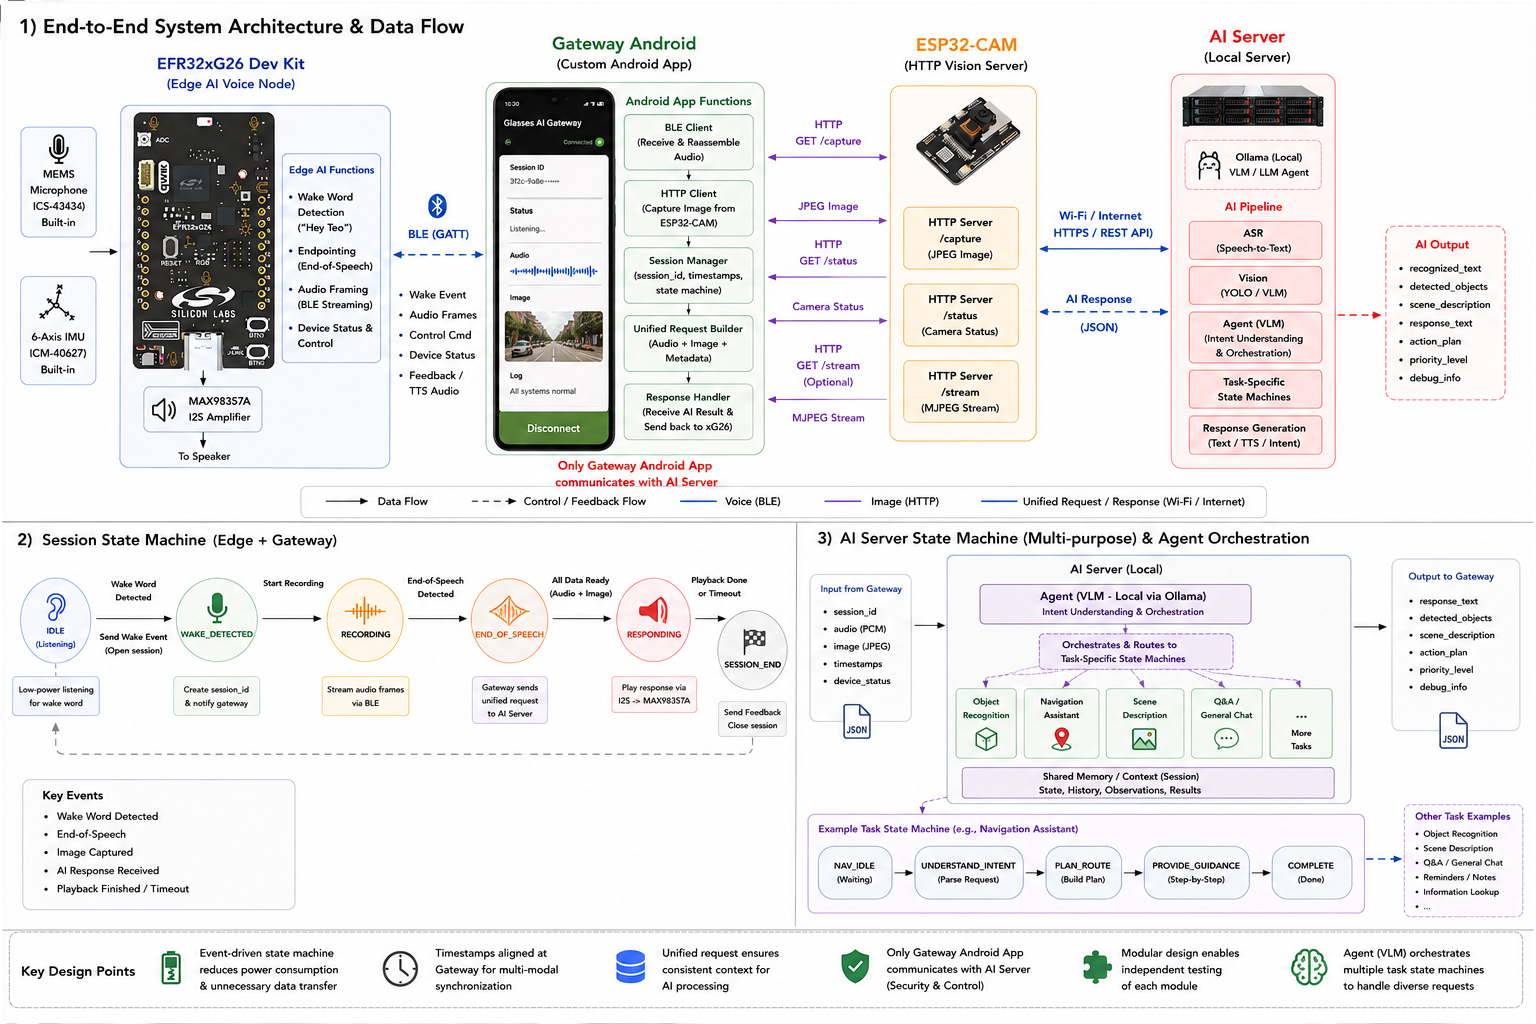
\includegraphics[width=0.76\textwidth]{uploads/so_do_6.png}
\caption{Vòng đời session tại gateway Android. Gateway nhận audio command từ EFR32xG26, lấy ảnh JPEG từ ESP32-CAM, gắn metadata thời gian, gửi request hợp nhất lên AI server và chuyển phản hồi về thiết bị đeo qua BLE.}
\end{figure}

Gateway Android đóng vai trò middleware trung tâm của toàn bộ hệ thống. Ứng dụng Android quản lý \texttt{session\_id}, đồng bộ timestamp giữa audio và image, sau đó tạo unified request chứa audio, image và metadata để gửi lên AI server.

Tại AI server, audio command được xử lý bằng ASR để tạo \texttt{recognized\_text}, trong khi ảnh JPEG được đưa qua YOLO hoặc Vision Language Model để tạo \texttt{detected\_objects} và \texttt{scene\_description}. Một VLM được host cục bộ bằng Ollama đóng vai trò agent điều phối giữa các state machine tác vụ như hỗ trợ tìm vật thể, mô tả ngoại cảnh hoặc hướng dẫn di chuyển.

Sau khi xử lý hoàn tất, AI server trả về \texttt{response\_text} cho gateway Android. Nội dung phản hồi tiếp tục được gửi qua BLE tới EFR32xG26 để phát âm thanh thông qua MAX98357A và loa ngoài. Khi phiên kết thúc, state machine quay lại trạng thái \texttt{IDLE} để tiếp tục lắng nghe wake word cho phiên tiếp theo.

Tổng thể, vòng đời của một phiên tương tác có thể mô tả như sau:

\begin{center}
\texttt{
IDLE
$\rightarrow$
WAKE\_DETECTED
$\rightarrow$
RECORDING
$\rightarrow$
PROCESSING
$\rightarrow$
RESPONDING
$\rightarrow$
IDLE
}
\end{center}
\section{Nguồn lực, phân công và mốc tiến độ}
Việc phân công được bám theo bốn hướng triển khai chính: điều phối và thiết kế hệ thống, nhúng EFR32xG26, app gateway Android và AI server. Các đầu việc được gắn trực tiếp với từng thành viên để tránh chồng chéo trách nhiệm và giúp quá trình tích hợp toàn chuỗi dễ theo dõi hơn. Do các module có thể phát triển song song, tiến độ được tổ chức theo từng hạng mục chạy đồng thời và chốt mốc hoàn thiện toàn diện trong tháng 9.

\begin{table}[H]
\centering
\caption{Phân công nhiệm vụ theo thành viên.}
\small
\begin{tabularx}{\textwidth}{p{3.0cm}p{3.8cm}Y}
\toprule
\textbf{Thành viên} & \textbf{Phụ trách chính} & \textbf{Nhiệm vụ và đầu ra} \\
\midrule
Hà Đức Khôi & Trưởng nhóm, thiết kế khung phần cứng và AI & Chốt kiến trúc tổng thể, điều phối tích hợp, thiết kế bố trí gọng kính/khung gá phần cứng, xây dựng AI Processing API, agent Ollama và các state machine theo tác vụ. Đầu ra là kiến trúc hệ thống, khung phần cứng nguyên mẫu và pipeline AI server. \\
Nguyễn Hương Giang & Nhúng EFR32xG26: wake word và endpointing & Triển khai pipeline TinyML trên xG26, lấy mẫu microphone, phát hiện wake word ``Hey Tèo'', xác định điểm kết thúc câu nói và mở/đóng phiên audio ổn định. Đầu ra là node giọng nói hoạt động đúng vòng đời phiên. \\
Nguyễn Minh Cát & Nhúng EFR32xG26: BLE và phản hồi âm thanh & Phát triển BLE GATT, đóng gói audio frame có \texttt{sequence\_number}, nhận feedback command từ gateway và phát phản hồi qua I2S/MAX98357A. Đầu ra là luồng truyền audio và phản hồi hai chiều giữa xG26 và gateway. \\
Kiểu Nhật Linh & App gateway Android & Code app Android để quản lý \texttt{session\_id}, timestamp, BLE với xG26, HTTP tới ESP32-CAM, gửi request hợp nhất lên AI server và chuyển phản hồi về thiết bị đeo. Đầu ra là app gateway Android hoạt động toàn chuỗi. \\
\bottomrule
\end{tabularx}
\end{table}

\begin{table}[H]
\centering
\caption{Tiến độ thực hiện theo hạng mục từ tháng 5 đến tháng 9.}
\small
\setlength{\tabcolsep}{4pt}
\renewcommand{\arraystretch}{1.18}
\begin{tabularx}{\textwidth}{p{3.0cm}p{2.2cm}Y p{3.0cm}}
\toprule
\textbf{Hạng mục} & \textbf{Thời gian thực hiện} & \textbf{Nội dung chính} & \textbf{Mốc hoàn thành} \\
\midrule
Chốt kiến trúc tổng thể & Tháng 5 & Xác định luồng xG26--Android--ESP32-CAM--AI server, chuẩn hóa \texttt{session\_id}, API schema, endpoint và state machine sơ bộ. & Hoàn thành tài liệu thiết kế hệ thống. \\
Khung phần cứng và bố trí module & Tháng 5--7 & Thiết kế, lắp thử và tinh chỉnh gọng kính; bố trí nguồn cấp, camera, microphone và loa để bảo đảm khả năng đeo thử. & Khung nguyên mẫu cố định đủ module. \\
Nhúng EFR32xG26 & Tháng 5--8 & Chuẩn hóa dữ liệu wake word, dựng pipeline TinyML; tích hợp wake word ``Hey Tèo'', endpointing, buffer audio, BLE frame có \texttt{sequence\_number} và phản hồi I2S/MAX98357A. & Firmware sẵn sàng tích hợp demo. \\
ESP32-CAM và HTTP Vision Server & Tháng 5--6 & Triển khai \texttt{/capture}, \texttt{/status}, \texttt{/stream}; ổn định capture JPEG, cấu hình Wi-Fi nội bộ và kiểm thử độ trễ cơ bản. & Camera server hoàn thiện sớm để ghép với gateway từ tháng 6. \\
App gateway Android & Tháng 5--8 & Dựng UI trạng thái, quản lý \texttt{session\_id}, tích hợp BLE với xG26, HTTP với ESP32-CAM, tạo request hợp nhất, log timestamp và retry policy. & App điều phối được một phiên hoàn chỉnh. \\
AI server và agent Ollama & Tháng 5--8 & Hoàn thiện pipeline ASR/YOLO/VLM, tích hợp VLM local qua Ollama, xây agent điều phối, fallback và log debug cho các tác vụ chính. & API trả phản hồi ổn định cho gateway. \\
Tích hợp và kiểm thử toàn chuỗi & Tháng 7--9 & Ghép đủ các node trong một phiên, chạy lặp lại kịch bản mô tả cảnh, tìm vật thể và hướng dẫn đường đi; đo latency, độ ổn định và sửa lỗi liên thông. & Hoàn thiện demo và chuẩn bị bảo vệ. \\
\bottomrule
\end{tabularx}
\end{table}




\section{Kết quả \& tiến độ hiện tại của triển khai nguyên mẫu}
Phần này phản ánh đúng trạng thái hiện tại của nguyên mẫu thay vì trình bày như một hệ thống đã ghép đủ bốn nút. Tính đến thời điểm viết báo cáo, nhóm đã hoàn thành một phiên bản thô cho kịch bản hỗ trợ lấy vật thể. Ở phiên bản này, ESP32-CAM chụp ảnh và gửi trực tiếp dữ liệu lên AI server; server xử lý ảnh, xác định vật thể mục tiêu trong khung hình và tạo phản hồi hướng dẫn ở mức thử nghiệm. Luồng này giúp nhóm kiểm chứng trước phần thị giác và AI trước khi bổ sung gateway Android và node EFR32xG26.

Ngoài phần hình ảnh, luồng voice thử nghiệm cũng được tổ chức theo hướng gửi trực tiếp lên server. Âm thanh được thu từ microphone INMP441 gắn với ESP, sau đó ESP gửi dữ liệu âm thanh thẳng lên AI server để thực hiện STT (Speech-to-Text). Server dùng nội dung câu lệnh đã nhận dạng kết hợp với ảnh từ ESP32-CAM để xử lý kịch bản hỗ trợ lấy vật thể, rồi sinh câu trả lời và thực hiện TTS (Text-to-Speech). Phản hồi âm thanh được gửi ngược lại để phát ra loa theo module loa đã đề cập ở mục phần cứng, cụ thể là hướng phát qua I2S/MAX98357A.

Hiện tại, EFR32xG26 và ứng dụng gateway Android chưa được tích hợp vào luồng chạy thực tế. Vì vậy, demo hiện tại chưa bao gồm wake word ``Hey Tèo'', endpointing, BLE GATT, quản lý \texttt{session\_id} trên app Android hay phát phản hồi âm thanh qua EFR32xG26. Các thành phần này vẫn giữ vai trò trong kiến trúc cuối, nhưng sẽ được tích hợp sau khi luồng ESP--AI server đủ ổn định.

\begin{center}
\texttt{ESP32-CAM/ESP + INMP441 $\rightarrow$ AI SERVER (STT + Vision + TTS) $\rightarrow$ Loa I2S/MAX98357A}
\end{center}

\begin{table}[H]
\centering
\caption{Tiến độ hiện tại của nguyên mẫu.}
\small
\begin{tabularx}{\textwidth}{p{3.0cm}p{2.4cm}Y Y}
\toprule
\textbf{Hạng mục} & \textbf{Trạng thái hiện tại} & \textbf{Phần đã có} & \textbf{Việc tiếp theo} \\
\midrule
Kính thô thực tế & Đã có bản thô & Đã lắp thử dạng kính để đặt camera và kiểm tra hướng nhìn thực tế của nguyên mẫu. & Cố định lại module, tối ưu dây nối, nguồn cấp và vị trí đeo. \\
ESP32-CAM & Đã chạy thô & Chụp ảnh từ camera và gửi trực tiếp dữ liệu lên AI server trong kịch bản thử nghiệm. & Ổn định Wi-Fi, nguồn cấp, góc nhìn camera và thời gian phản hồi. \\
AI server cho kịch bản lấy vật thể & Đã chạy thô & Nhận ảnh từ ESP32-CAM, xử lý kịch bản tìm/lấy vật thể và sinh hướng dẫn thử nghiệm cho người dùng. & Tinh chỉnh nhận diện vật thể, cách mô tả vị trí và phản hồi hướng dẫn. \\
Luồng ESP32-CAM--AI server & Đã có demo end-to-end thô & Luồng hiện tại đi trực tiếp từ ESP32-CAM lên server, dùng để chứng minh phần thị giác--AI hoạt động được trước. & Chuyển sang kiến trúc chuẩn qua app gateway Android để đồng bộ phiên. \\
EFR32xG26 & Chưa tích hợp vào demo hiện tại & Chưa có wake word, endpointing, BLE và phát phản hồi âm thanh trong luồng chạy thực tế. & Tích hợp node giọng nói, BLE GATT và phản hồi âm thanh sau bước demo thị giác--server. \\
App gateway Android & Chưa tích hợp vào demo hiện tại & Chưa quản lý \texttt{session\_id}, BLE với xG26, HTTP với ESP32-CAM và request hợp nhất lên AI server trong bản demo hiện tại. & Xây app gateway để thay thế luồng ESP32-CAM gửi thẳng lên server. \\
\bottomrule
\end{tabularx}
\end{table}

\textbf{Mã nguồn và hình ảnh hiện tại:} Mã nguồn demo hiện tại được đặt tại \href{https://github.com/NMC666/smart-glass}{repository GitHub của bản demo hiện tại}. Các hình dưới đây ghi lại demo chạy và ảnh kính thô thực tế của nguyên mẫu.

\begin{figure}[H]
\centering
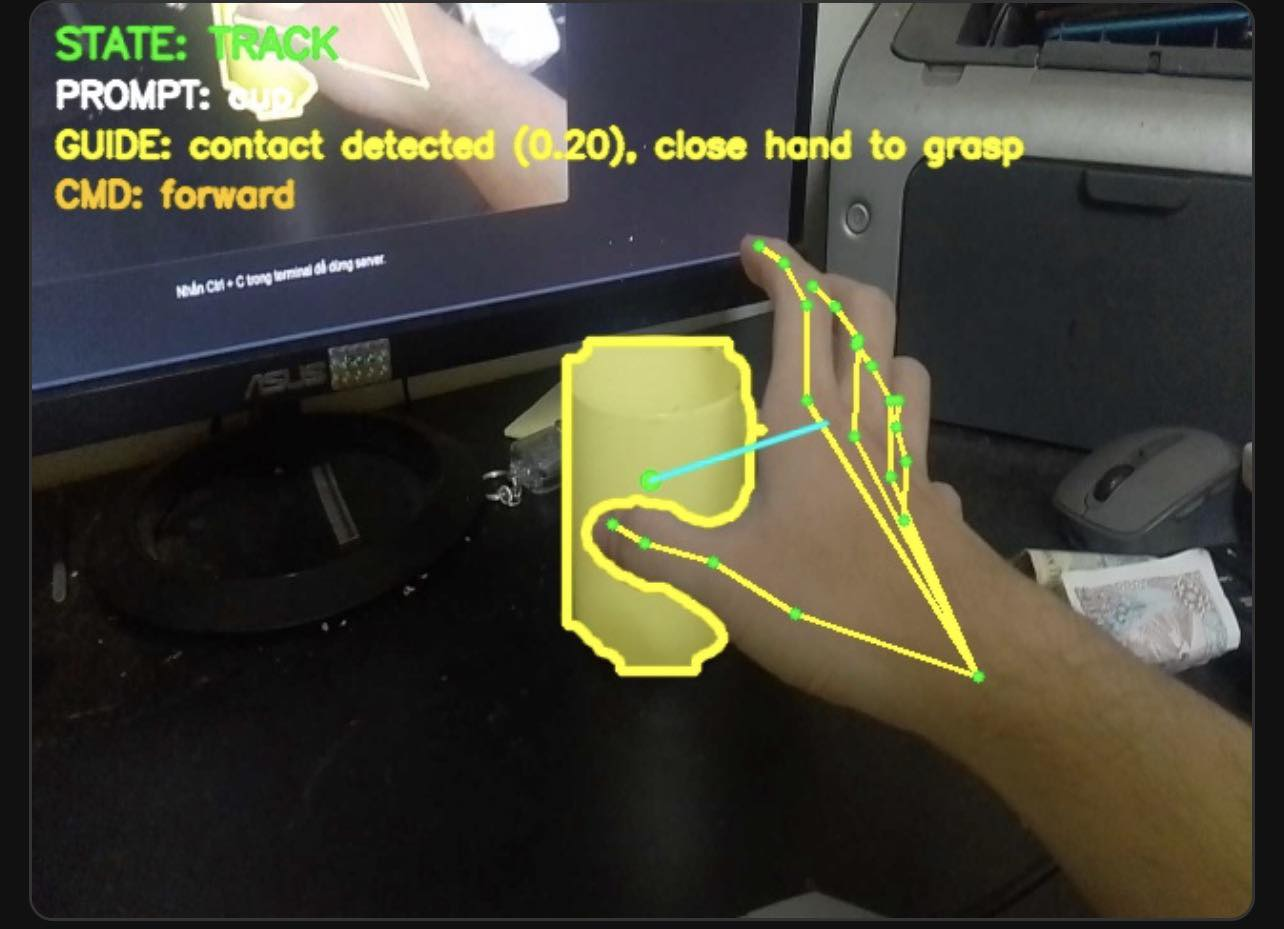
\includegraphics[width=0.76\textwidth]{uploads/demo_chay_lay_vat_the.jpg}
\caption{Demo chạy luồng ESP32-CAM gửi trực tiếp lên AI server cho kịch bản hỗ trợ lấy vật thể.}
\end{figure}

\begin{figure}[H]
\centering
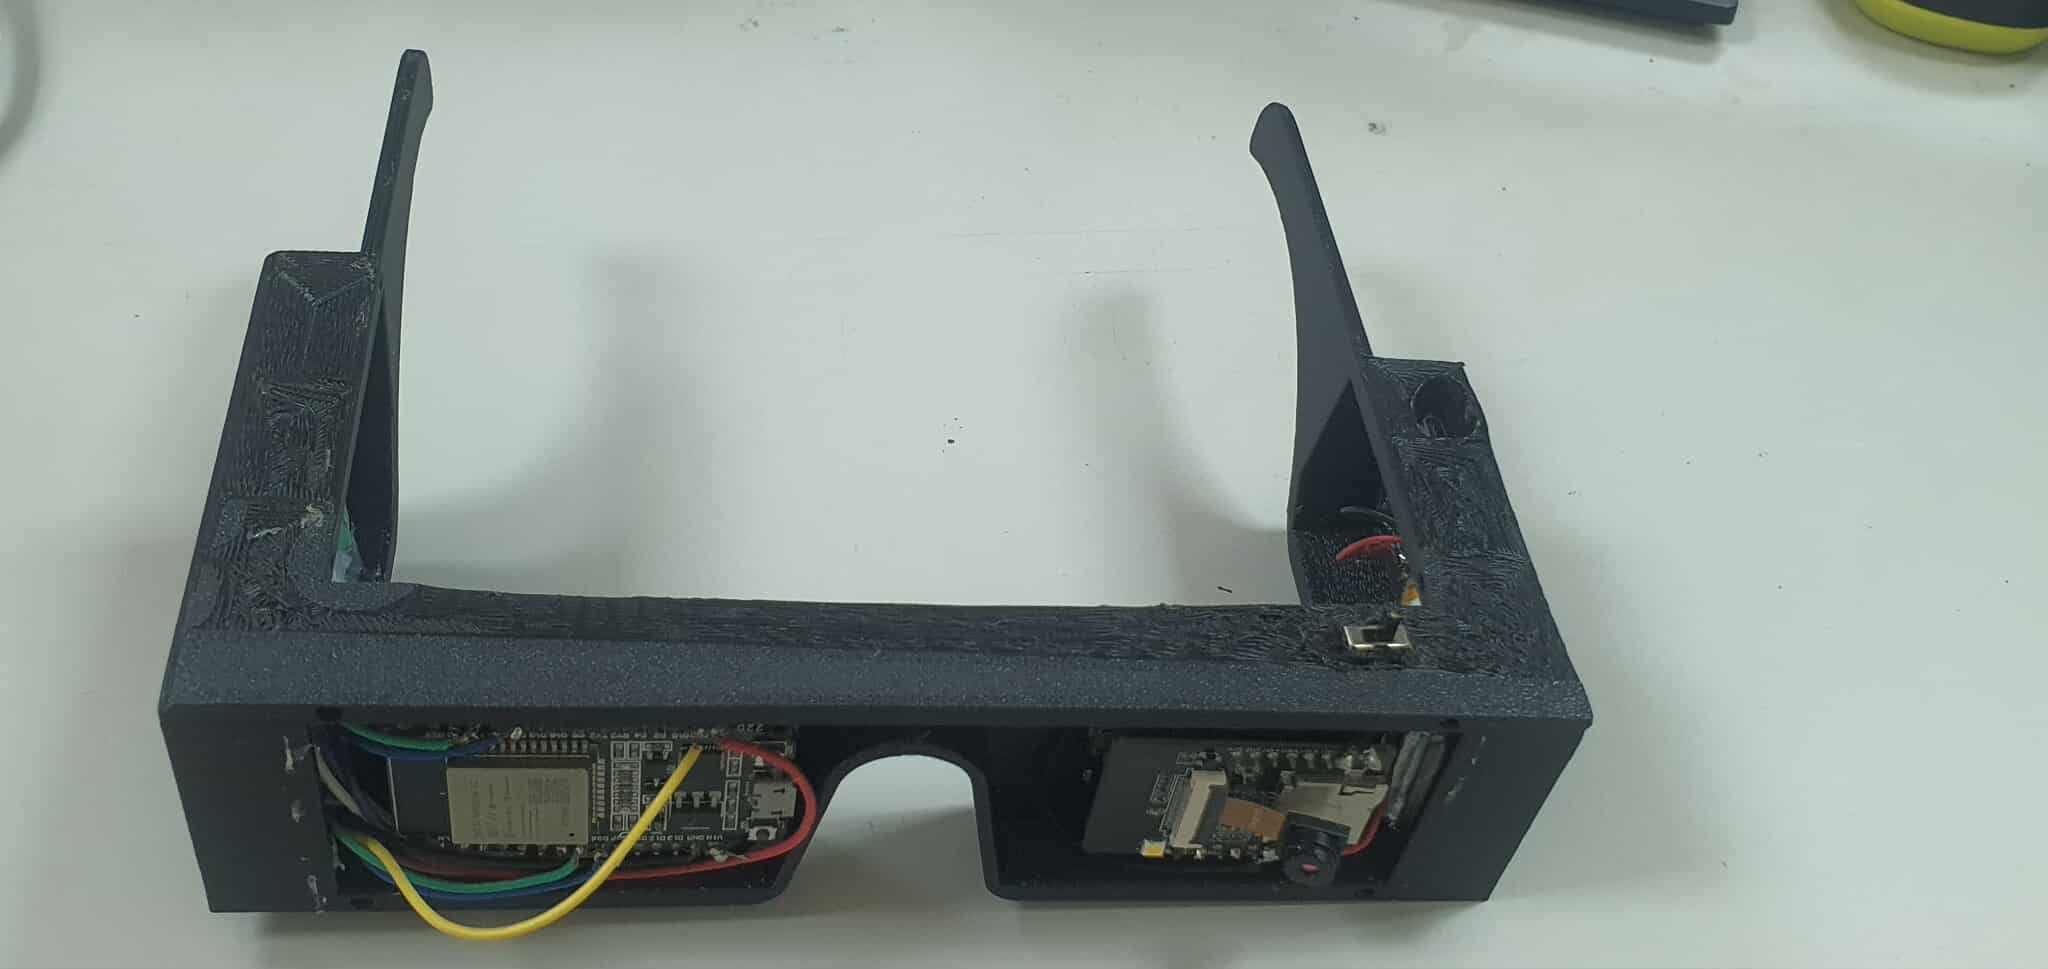
\includegraphics[width=0.76\textwidth]{uploads/kinh_tho_thuc_te.jpg}
\caption{Ảnh nguyên mẫu kính thô dùng để kiểm tra bố trí camera, hướng nhìn và khả năng đeo thử.}
\end{figure}



\section{Kết luận}
Dự án hướng tới một bài toán xã hội rõ ràng: hỗ trợ người khiếm thị nhận biết môi trường gần bằng một hệ thống đeo được có khả năng tiếp nhận lệnh bằng giọng nói và phản hồi bằng âm thanh. Kiến trúc nhiều nút đã được định hình với vai trò cụ thể cho EFR32xG26, ESP32-CAM, gateway Android và AI server. Mỗi thành phần xử lý một lớp dữ liệu riêng, nhưng cùng tham gia vào một chuỗi phiên thống nhất từ wake word đến phản hồi âm thanh.

Với cách tổ chức này, nguyên mẫu bám trực tiếp các tiêu chí Wireless Technology, Edge AI, IoT/Embedded và AI. Báo cáo đã xác định luồng kỹ thuật, giao thức truyền thông, tiến độ hiện tại và minh chứng demo thô cho kịch bản hỗ trợ lấy vật thể. Đây là nền tảng phù hợp để nhóm tiếp tục tích hợp EFR32xG26, app gateway Android, đo kiểm toàn chuỗi và chuẩn bị phần trình diễn trong khuôn khổ cuộc thi.

\end{document}
